\documentclass[a4paper,10pt]{article}
%\documentclass[a4paper,10pt]{scrartcl}

\usepackage[utf8]{inputenc}
\usepackage{graphicx}
\usepackage[demo]{graphicx}
\usepackage{caption}
\usepackage{subcaption}


\title{Introduction to machine learning}
\author{}
\date{}

\pdfinfo{%
  /Title    ()
  /Author   ()
  /Creator  ()
  /Producer ()
  /Subject  ()
  /Keywords ()
}

\begin{document}
\maketitle Introduction to machine learning, Extra project

Ensimmäisenä tehtävä oli luoda perceptron algoritmi, jota sitten käytetään käsinkirjoitettujen numeroiden luokitteluun. Tässä tapauksessa tarkoituksena
oli luokitella ainoastaan 1 ja 0. Tein toteutuksen Matlabilla. Tein numeroiden lataamiseen oman scriptin, joka valitsee numeroista vain 1 ja 0, 
ja jakaa pikselidatan sekä oikeat luokat omiin muuttujiinsa. Tämän lisäksi on itse perceptron funktio omassa tiedostossaan, joka hoitaa luokittelijan
opettamisen. Sitten on vielä classifier funktio, jolla voi luokitella käyttäen aiemmin luotua luokittelijaa. 

Ensimmäisenä tein 2-uloitteisia testiaineistoja, jotta tiedän toimiiko luokittelija. Kaikissa seteissä pisteitä oli senverran vähän että jos 
luokat olivat eroteltavissa, niin algoritmi konvergoi parissa iteaatiossa. Seuraavalla sivulla muutamia kuvia, joista näkee minkälaisia 
ryhmiä luokittelija sai luotua. Kohtasin pieniä ongelmia siinä miten olisin saanut MatLabissa esitettyä pisteet omina luokkinaan, mutta 
tässä tapauksessa onneksi pisteitä on niin vähän, että on melko selvää mitkä pisteet kuuluvat mihinkin luokkaan. Tarkastin kuitenkin käsin, että 
saadut tulokset olivat järkeviä.
\begin{figure}[ht!]

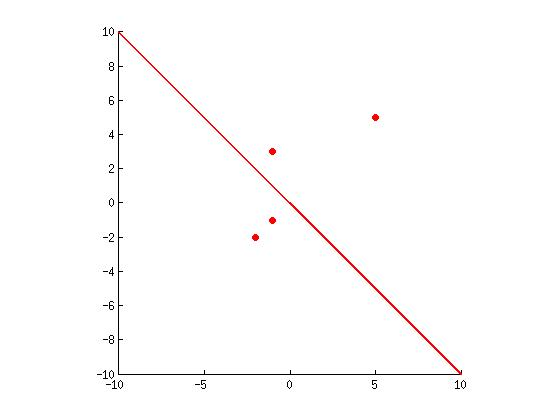
\includegraphics[width=70mm]{sanityCheck1.jpg}
\caption{Luokittelijan testi 1}


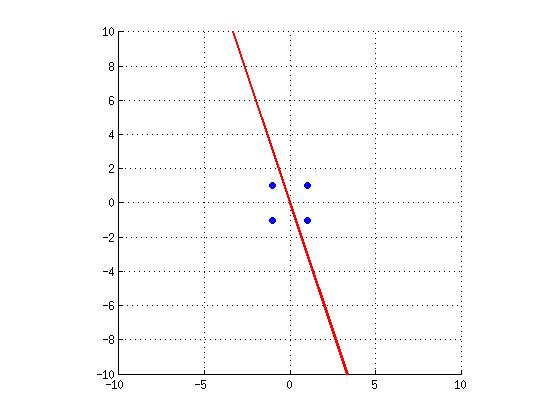
\includegraphics[width=70mm]{sanityCheck2.jpg}
\caption{Luokittelijan testi 2}

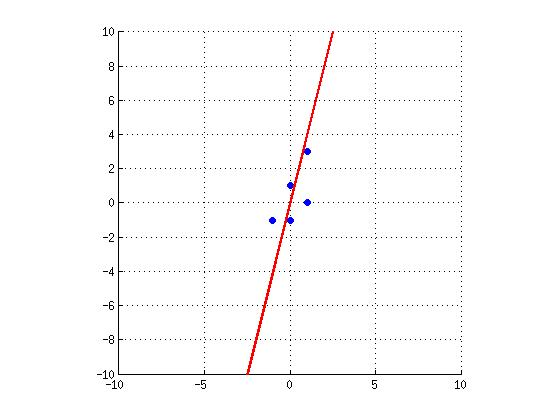
\includegraphics[width=70mm]{sanityCheck3.jpg}
\caption{Luokittelijan testi 3, Kaikista toimivista luokista tässä oli pienin marginaali.}

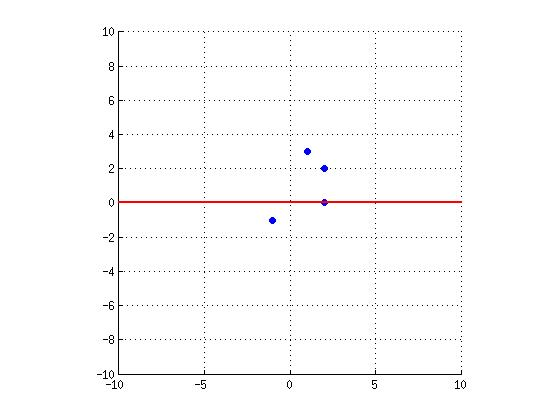
\includegraphics[width=70mm]{sanityCheck4.jpg}
\caption{Pisteet eivät olleet luokiteltavissa, algoritmi ei konvergoinut}

\label{overflow}
\end{figure}



Seuraavaksi latasin apufunktiolla 5000 datapistettä mnist aineistosta ja otin sieltä vain 1 ja 0.
Opetusaineistoon ja testiaineistoon tuli kumpaankin noin 500 alkiota. Perceptron algoritmi konvergoi toisella iteraatiolla. Tämän jälkeen kun luokittelijan
antoi syötteenä testiaineistolle, oli virheprosentti 0\%.
Tulos ei sinällään ollut kovin yllättävä, koska aineiston dimensio oli todella suuri, sekä 1 ja 0 ovat melko kaukana toisistaan jos asiaa miettii 
pikselitasolla. 

\end{document}
